\documentclass[11pt,a4paper]{article}
\usepackage[utf8]{inputenc}
\usepackage[T1]{fontenc}

\usepackage[margin=3cm]{geometry}
\usepackage{microtype}

\usepackage[fleqn]{amsmath}
\usepackage{amsfonts}
\usepackage{amssymb}
\usepackage{color}
\usepackage{lscape}
\usepackage{graphicx}

\title{Turbulent Flow Simulation, 2nd Sheet Report}
\author{Peter Münch, Walter Simson, Marten Lienen}

\begin{document}

\newcommand{\abl}[2]{\frac{\partial \, #1}{\partial \, #2}}
\newcommand{\abll}[2]{\frac{\partial^2 \, #1}{\partial \, #2^2}}
\newcommand{\ave}[1]{\left\langle#1\right\rangle}
\newcommand{\new}[1]{\textcolor{red}{#1}}

\maketitle

\section{Parallelization}

\subsection{MPI}

We have implemented the communication of flow quantities as explained in a
Berkeley paper on ghost
cells\footnote{\emph{http://parlab.eecs.berkeley.edu/wiki/\_media/patterns/ghostcell.pdf}}
and illustrated in figure \ref{fig:border-exchange}. The general approach is as follows

\begin{itemize}
\item First we exchange the flow quantity with the neighbors in one direction spare the corners respectively edges
\item In the second phase we exchange in another direction but include the corners
\item For a 3D simulation we finally exchange values in the third direction and include the remaining edge
\end{itemize}

This incremental sending of more edge values ensures that you send the minimal
amount of data to update all ghost layer.

A quite general implementation can be found in \textsc{MPICommunicator} that can
be reused for different quantities, data types and ghost layer widths.

\begin{figure}[h]
  \centering
  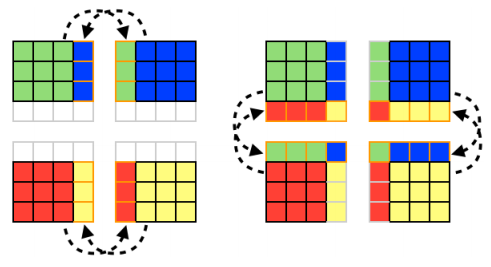
\includegraphics[width=\textwidth]{border-exchange}
  \caption{Two Dimensional Border Exchange}
  \label{fig:border-exchange}
\end{figure}

\subsection{Validation}

We compared simulation results obtained with different domain decompositions and
they were identical up to the 8th decimal place.

\section{Scaling and Parallelisation}
\subsection{Scalabilty}

As expected, linear scalability was not achieved, never the less, the overall
scalability of our implementation was satisfactory inversely quadratic when
scaled "strongly". Our weak scaling implementation also achieved an almost
constant running time and thus speed up when the PETSc solver was ignored. It
should be noted, that the PETSc solver generally did not scale well, most likely
due to insufficient PETSc-tuning. We therefore also observed the execution time
of our NS solver both with and without the PETSc overhead.

Figure \ref{fig:scaling-channel-strong} presents the analysis of a strong
scaling experiment with a channel flow configuration. Most importantly one can
see that the total speedup scales roughly linearly with the number of processes
and a slope of about $0.5$. One can observe that the ratio of communication time
rises abruptly from 16 to 20 processes. This exemplifies the advantageousness of
keeping communication local to a node and avoiding network traffic and the size
of the performance loss that can result when a job does not fit the used
nodes. Since we have limited influence on the performance of the PETSc solver
itself we have also plotted the speedup of everything \emph{except} PETSc. This
scales nicely as well but has two notable dips at 36 and 52 nodes. These result
from the fact 36 is split into $9$ times $4$ and 52 into $13$ times $4$
processes along the X and Y axis, which stretch the cells and lead to a worse
ratio of volume to surface area.

Figure \ref{fig:scaling-channel-weak} shows the analysis of a weak scaling
experiment with a channel scenario. The total speedup graph shows that we have
scaled the work per process linearly.

\begin{figure}[h]
  \centering
  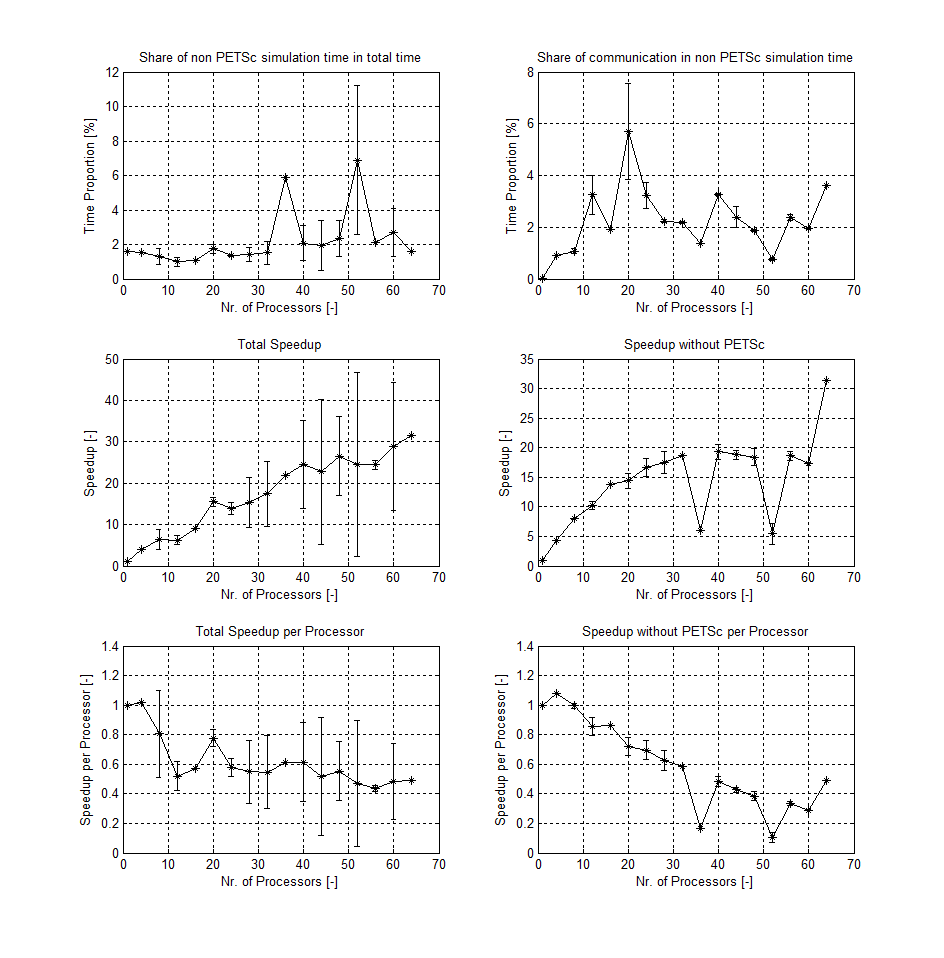
\includegraphics[width=\textwidth]{scaling/channel-strong}
  \caption{\emph{Strong} scaling experiment with a channel scenario}
  \label{fig:scaling-channel-strong}
\end{figure}

\begin{figure}[h]
  \centering
  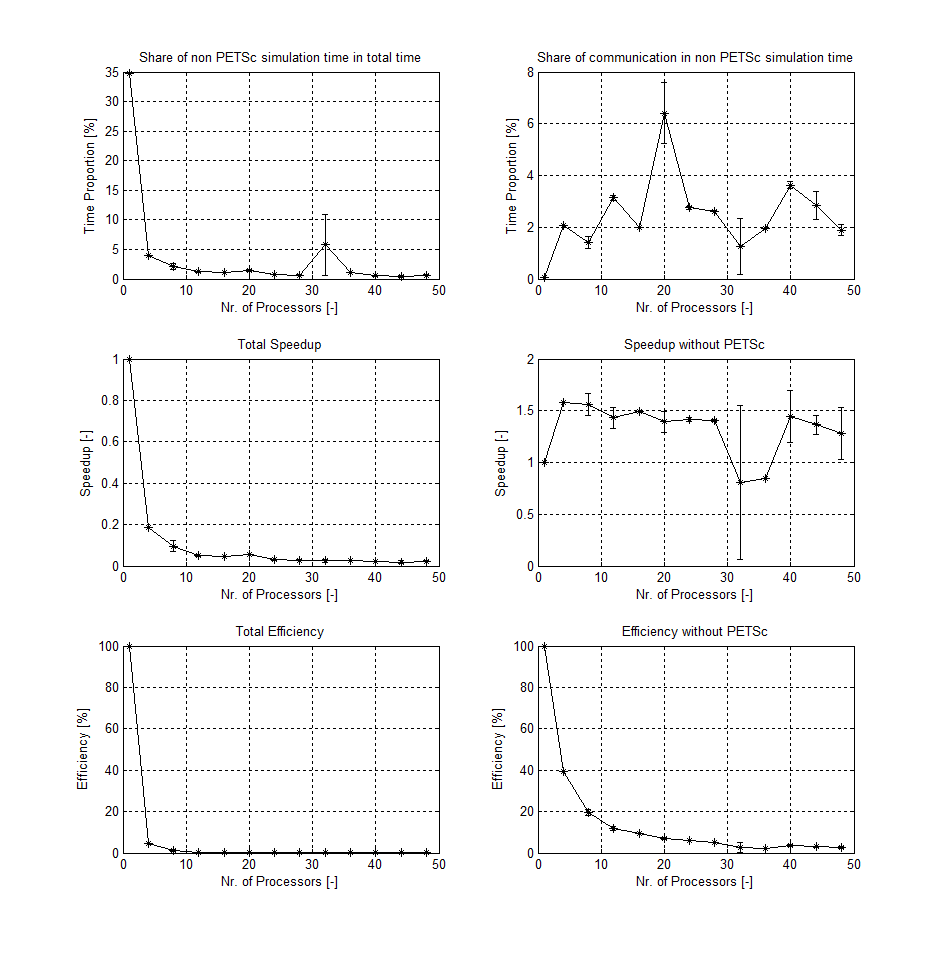
\includegraphics[width=\textwidth]{scaling/channel-weak}
  \caption{\emph{Weak} scaling experiment with a channel scenario}
  \label{fig:scaling-channel-weak}
\end{figure}

\clearpage

\section{RANS (Eddy viscosity model)}
\subsection{Equations to solve}

Turbulent flow can be described with the (incompressible) RANS-equations:

\begin{align}
\abl{\ave{u_i}}{x_i}=0
\end{align}
\begin{align}
\abl{\ave{u_i}}{t}+\abl{\ave{u_i}\,\ave{u_j}}{x_j}=-\frac{1}{\ave{\rho}}\,\abl{P}{x_i}+2\,\new{\abl{}{x_j}\left( \left(\nu+\nu_T\right)\,S_{ij} \right)}+f_i
\\\qquad\text{with: }\frac{\ave{P}}{\rho}=\frac{\ave{p}}{\rho}+\frac{2}{3}\,K
\quad \text{and}\quad
S_{ij}=\frac{1}{2}\left(\abl{u_i}{x_j}+\abl{u_j}{x_i}\right)
\nonumber
\end{align}
%\begin{align}
%\abl{\ave{u_j}}{x_i}\abl{\ave{u_i}}{x_j}=-\abl{}{x_i}\left( \frac{1}%{\rho}\abl{P}{x_i} \right)	\qquad\text{with: }P=\ave{p}+\frac{2}{3}\rho\,K
%\end{align}
The red highlighted term indicates the difference to the incompressible Navier-Stokes-equations. While we directly solve NS for pressure, when using RANS we receive the sum of pressure and the TKE-term ($\ave{P}/\rho$).

\subsection{Algorithm}\label{sec:algorithm}
Following steps are performed in our program to solve the RANS with the help of the algebraic turbulence model:
\begin{itemize}
\item[1.] Calculate $\Delta t$:
\begin{align}
\Delta t < \min\left\lbrace
\frac{\left( Re^{-1}+\nu_t \right)^{-1}}{2}\left(
\frac{1}{\Delta x^2}+
\frac{1}{\Delta y^2}+
\frac{1}{\Delta z^2}
\right)^{-1}
,
\frac{\Delta x}{|u_{max}|},
\frac{\Delta y}{|v_{max}|},
\frac{\Delta z}{|w_{max}|}
\right\rbrace
\end{align}
\item[2.] Calculate $F_i^\circ$:
\begin{align}
F_i^\circ=u_i^\circ+\Delta t\left(-\abl{u_i^\circ\,u_j^\circ}{x_j} +2\,\new{\abl{}{x_j} \left( \,\left(\nu+\nu_T^\circ\right)S_{ij}^\circ\right)}+f_i^\circ  \right)
\end{align}
The appendix shows the discrete form of the local derivatives necessary to express the red term.
\item[3.] Solve Pressure-Poission-Equation for $(p^+/\rho)$:
\begin{align}
\frac{1}{\Delta t} \abl{F_i^\circ}{x_i}  =
\frac{\partial^2 (p^+/\rho)}{\partial x_i\,\partial x_i}
\end{align}
\item[4.] Calculate velocities $u_i^+$:
\begin{align}
u_i^+
=F_i^\circ-\frac{\Delta t}{\rho}\,\abl{(p^+/\rho)}{x_i}
\end{align}
\item[5.] Calculate eddy viscosity $\nu_T^+$ and communicate values with MPI:
\begin{align}
\nu_{t}=l_m^2\sqrt{2\,S_{ij}\,S_{ij}}\quad\text{with} \quad l_m=min(0.41\,h;0.09\,\delta)
\end{align}
\item[6.] Calculate additional useful variables: velocity fluctuation $u'$ and pressure $p$:
\begin{align}
u'=l_m\sqrt{2\,S_{ij}\,S_{ij}}\qquad\qquad
\frac{\ave{p}}{\rho}=\frac{\ave{P}}{\rho}-\frac{2}{3}\,K=\frac{\ave{P}}{\rho}-u'u'
\end{align}
\end{itemize}

\clearpage
\subsection{Implementation}
These thoughts lead us to:

\begin{itemize}
\item A new FlowField-Class \textsc{FlowFieldTurbA} was created (based on the Adapter/Decorator Pattern), which has an instance of a laminar flow field and implements the \textsc{FlowField}-interface. The created flow field has addtional scalar fields (vortex viscosity $\nu_t$, local distance to the nearest wall $h$, mixing length $l_m$, velocity variation $u'$).
\item A new implementation of the Simulation-interface was created: \textsc{SimulationTurbA}. It incorporates the algorithm described in section~\ref{sec:appendix}. It uses the newly created stencils (\textsc{NutStencil}, \textsc{FGHStencilTurb}).
\item For the purpose of measuring the shortest distance from the middlepoint of a cell to a wall, the \textsc{WallDistanceManager} was written. It is called for each cell from the \textsc{HStencil} at the initialising of the turbulent simulation. WallDistanceManager is using the library ANN, which saves the coordinate of each wall-cell in a k-d tree, enabling to find the nearest wall cell in $\sim\ln(n)$-steps (with n = number of wall cells). We performed test simulations, in which we could confirm the performance.

\begin{figure}[h]
    \centering
    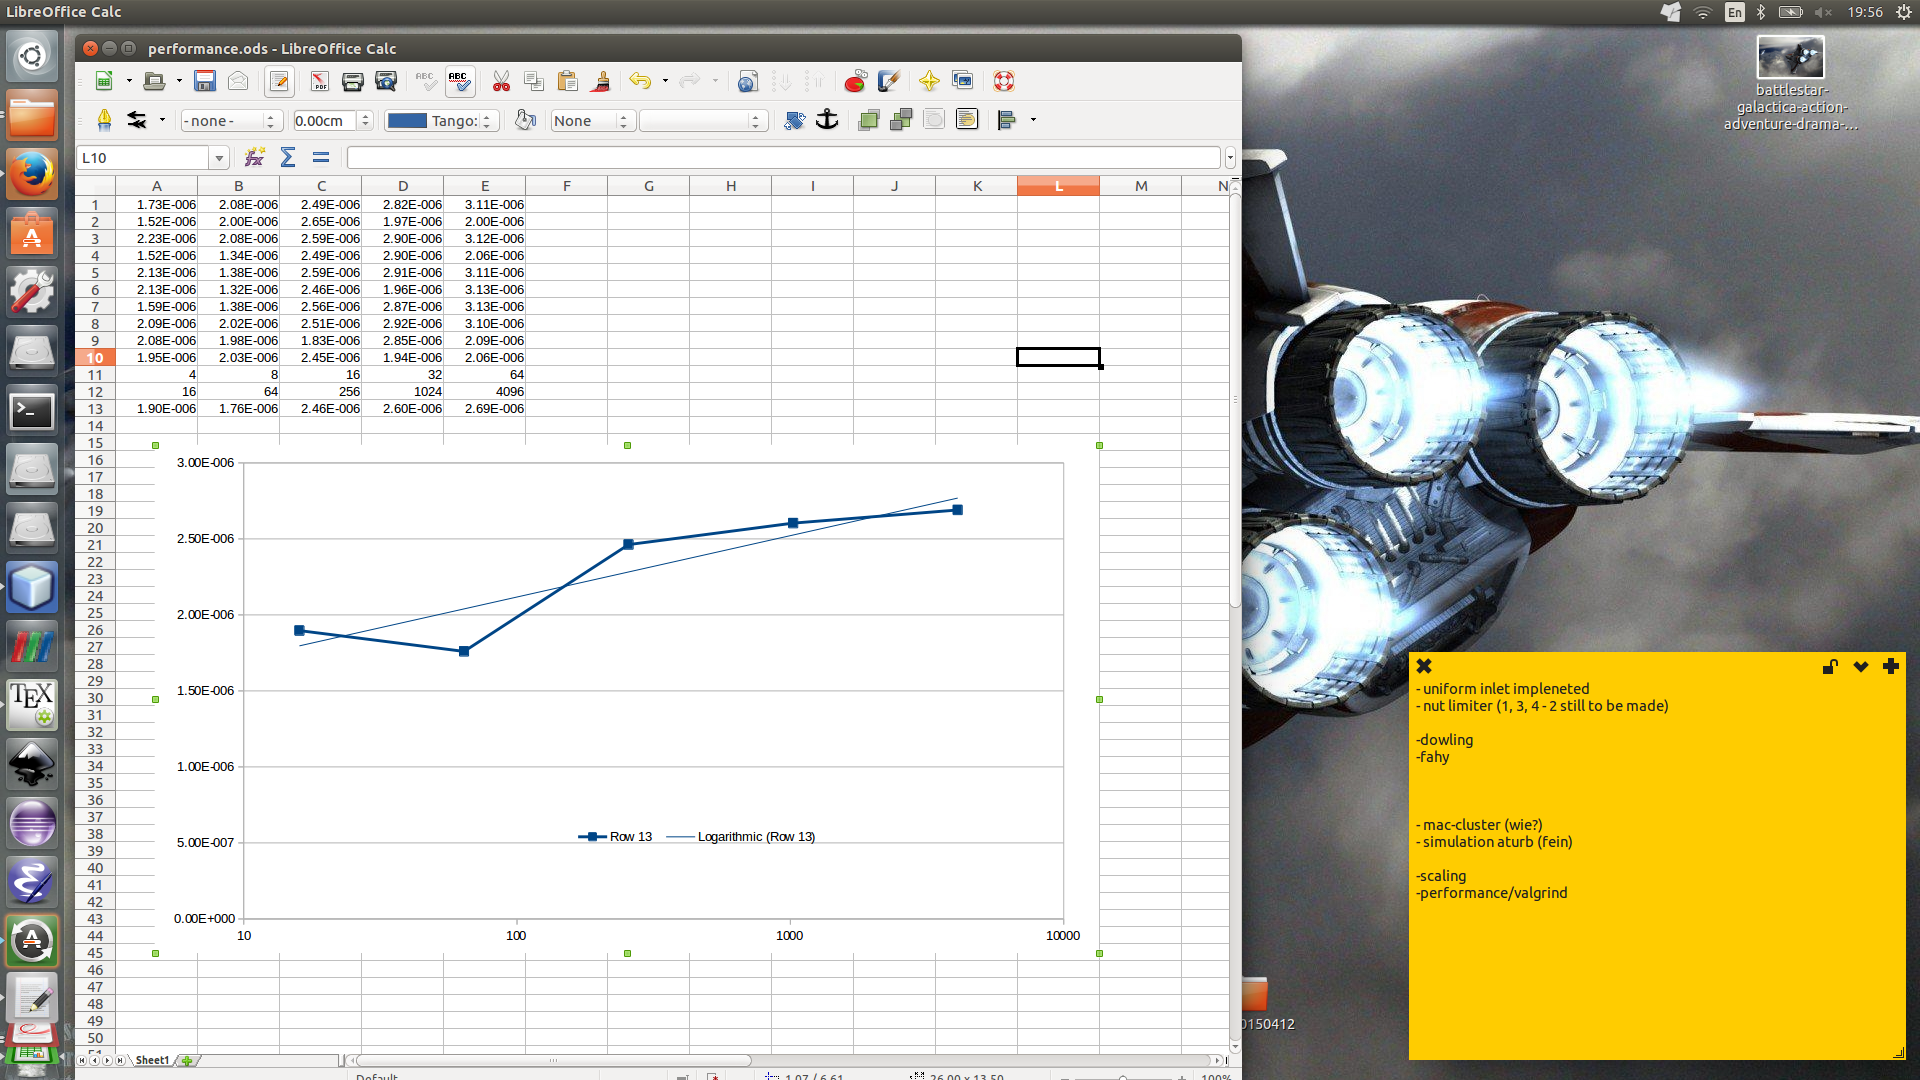
\includegraphics[width=0.8\textwidth]{ann}
    \caption{\textsc{WallDistanceManager}-perfomance test}
    \label{fig:vels}
\end{figure}

\item The VTK-Manager and the \textsc{MPICommunicator} were expanded to save and to communicate the additional variables respectively (Strategy Pattern).
\end{itemize}




\clearpage


\subsection{Results}
Different cases (laminar, turbulent with Re=100, with Re=1000 and with Re=5600 without $\nu_t$-limitation) of channel flow were performed under following conditions:
\begin{itemize}
\item constant uniform inlet velocity profile of $u=1m/s$
\item 2D-channel with the dimensions 25m$\times$1m
\item cell numbers 128$\times$128 and domain decomposition 2$\times$4.
\end{itemize}

\subsubsection{Velocities}
\noindent Figure~\ref{fig:vels} shows the u-velocity components along the cross section for each simulation case. The position of measurement and time were adjusted according to the case, so that the flow profile was stationary and fully developed.

\begin{figure}[h]
    \centering
    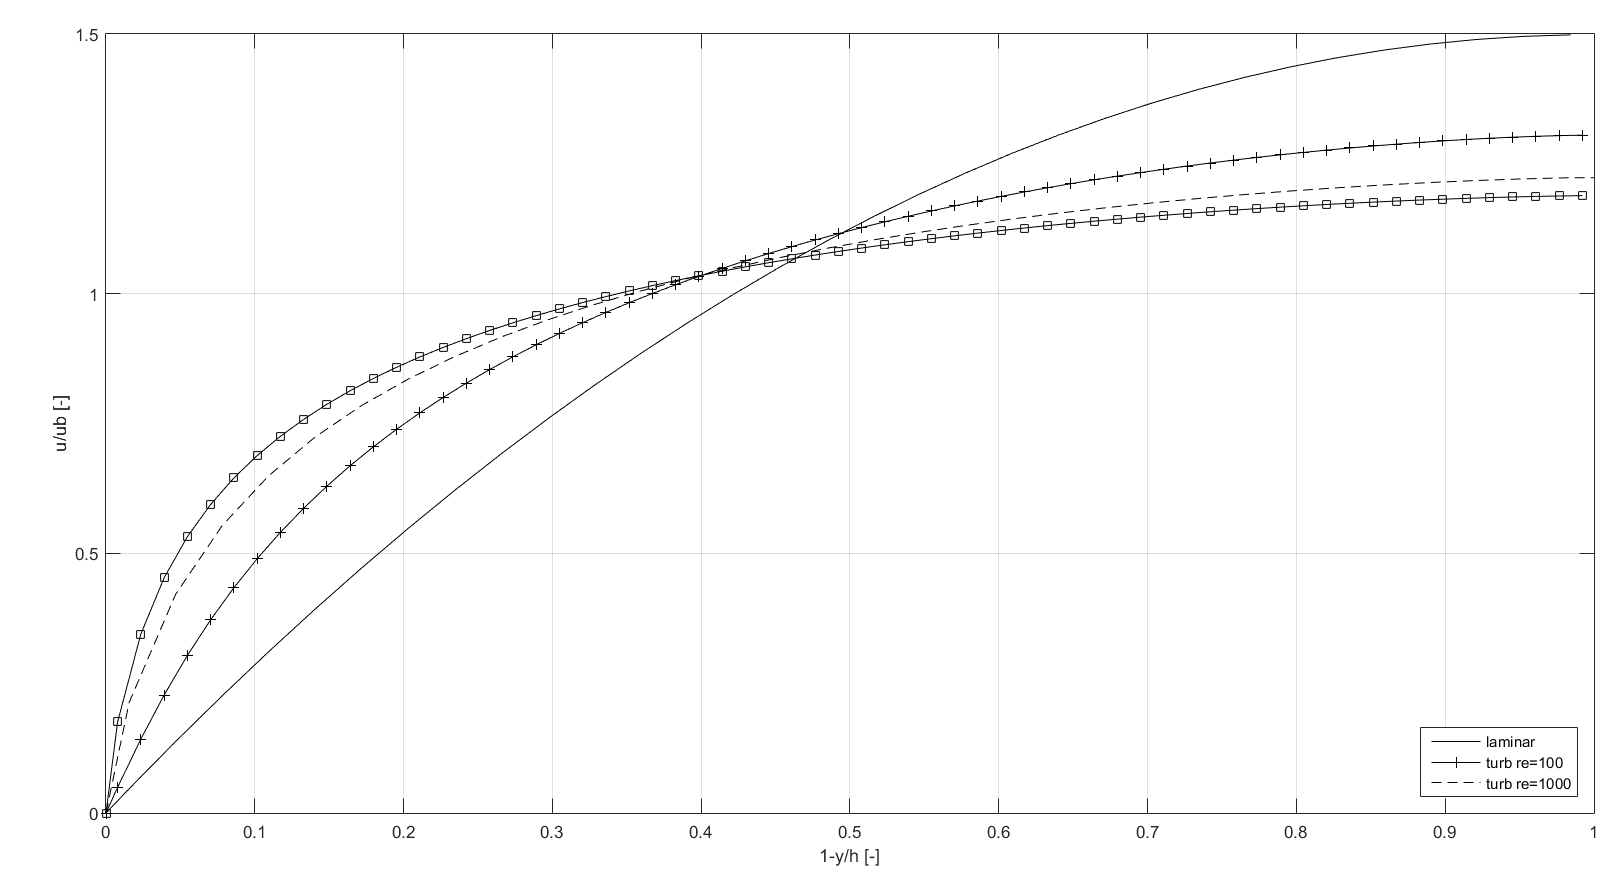
\includegraphics[width=1.0\textwidth]{velocities}
    \caption{Velocity profiles}
    \label{fig:vels}
\end{figure}

\noindent The velocities behave as expected. In the laminar case, the velocity profile has a parabolic form with a maximum of 1.5m/s. The turbulent simulations result in lower velocities (u$\le$1.5m/s): the higher the Reynolds-number the lower  the maximal velocity and the stouter the profile (the slope of the velocities is higher near the wall).

\subsubsection{Shear stress}

Figure~\ref{fig:taus} shows the shear stress profile along the cross section for each turbulent case. The shear stress components are normalized with $\tau_{net}=\tau_v+\tau_r$:

\begin{itemize}
\item viscous stress $\tau_v=\rho\nu\abl{\ave u}{y}$
\item Reynolds stress $\tau_r=-\rho\ave{u' v'}=\rho\nu_t\abl{\ave u}{y}$
\end{itemize}

\begin{figure}[h]
    \centering
    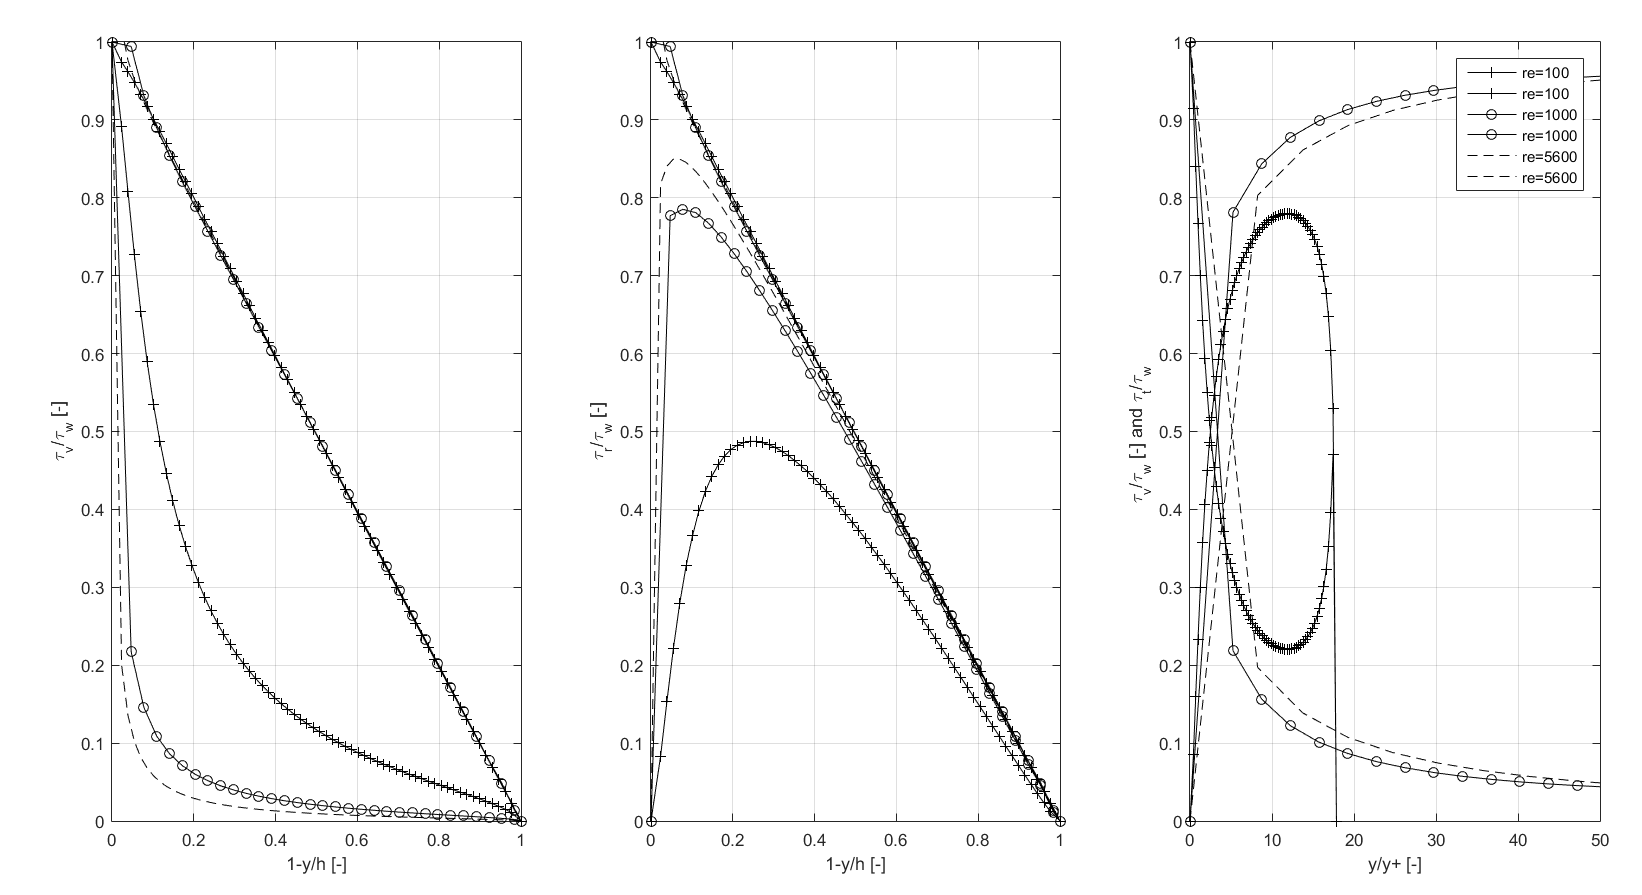
\includegraphics[width=1.0\textwidth]{tau}
    \caption{Viscous and Reynolds stresses}
    \label{fig:taus}
\end{figure}

\noindent Additionally the shear stress components are plotted over $y^+$. Self-similarity is clearly recognisable.

\subsubsection{Comparison with the literature}\label{sec:lit}
Following additional values have been calculated for the turbulent Re=5600 case.
\begin{align}
u_\tau=\sqrt{\tau_w/\rho}
\qquad\qquad
l^+=\nu/u_\tau
\qquad\qquad
Re_\tau=u_\tau\cdot\delta/\nu
\end{align}
Dimensionless dimensions were created with these and were compared to the measurement values from the literature [Kim, John; Moin, Parviz; Moser, Robert: Turbulence statistics in fully developed channel flow at low Reynolds number, in: J. Fluid Mech. (1987), vol. 177, p. 133-166]:

\begin{center}
\begin{tabular}{|l|c|c|c|}
\hline
 & Literature & Simulation & Simulation* \\\hline
$Re_\tau$ & 180 & 352 & 179\\\hline
$Re_c$ & 3300 & 3329 & 3329 \\\hline
$Re_m$ & 5600 & 5600 & 5600\\\hline
$u_m/u_\tau$ & 15.63 & 7.95 & 15.6\\\hline
$u_c/u_\tau$ & 18.20 & 9.45 & 18.6\\\hline
$u_c/u_m$ & 1.16 & 1.189 & 1.189\\\hline
$C_f = \tau_w / (0.5 \rho u_m^2)$ & 8.18$\times$10$^{-3}$ & 31.6$\times$10$^{-3}$ & 8.2$\times$10$^{-3}$\\\hline
\end{tabular}
\end{center}

\noindent The simulated maximal velocity $u_c/u_m$ matches well with the value from the literature. However, all the $\tau_w$-related variables ($Re_\tau$, $C_f$, $u_\tau$...) differ. Apparently $\tau_w$  was overestimated by a factor 3,86. The reason for this discrepancy is still unclear. If we decrease $\tau_w$ by 3,86, the simulated values (Simulation *) match well with the literature.

\newpage
\subsubsection{Sublayers}
Figure~\ref{fig:sublayers}-left shows the normalized velocity $w^+$  over $y^+$ and the expected velocity profile. They do not match. The reason for this is the discrepancy in simulated $\tau_w$ (neither $l^+$ and $u_{\tau}$ could be calculated the right way).


\begin{figure}[h]
    \centering
    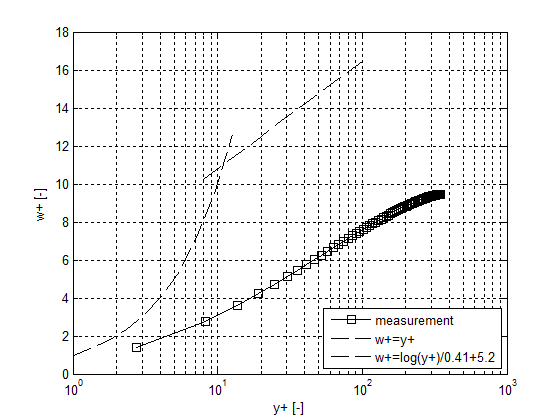
\includegraphics[width=0.49\textwidth]{wy1}
    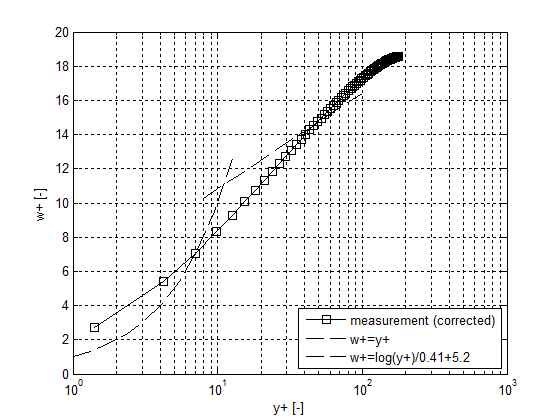
\includegraphics[width=0.49\textwidth]{wy2}
    \caption{Sublayers: $w^+$ over $y^+$}
    \label{fig:sublayers}
\end{figure}

\noindent Figure~\ref{fig:sublayers}-right shows a modified normalized velocity $w^+$ over $y^+$ . In this case, $l^+$ and $u_{\tau}$ was calculated with an adjusted $\tau_w$-value (as discussed in section~\ref{sec:lit}).

\subsubsection{Eddy viscosity limiter models}

Two different ways of limiting the eddy viscosity were implemented:
\begin{itemize}
\item[3.] compute the local boundary layer thickness by assuming a laminar flat plate Blasius boundary layer
\item[4.] compute the local boundary layer thickness by assuming a turbulent flat plate boundary layer.
\end{itemize}

\noindent Plot~\ref{fig:devel} shows the velocity profiles for different cross sections on the x-axis of different models (laminar, turbulent without $\nu_t$-limitation, turbulent with $\nu_t$-limitation 3 and 4). You can see that:
\begin{itemize}
\item The flow in the laminar simulation needs much longer to fully develop than in the case of the turbulent simulation without any limitation of eddy-viscosity.
\item $\nu_t$-limitation leads to faster development of the flow field. The maximal velocities are in the range of 10-16m higher than without any limitation (laminar-turbulent transition). It is expected that the maximal velocities will decrease to the values of the turbulent simulation with limitation.
\end{itemize}

\begin{figure}[h]
    \centering
    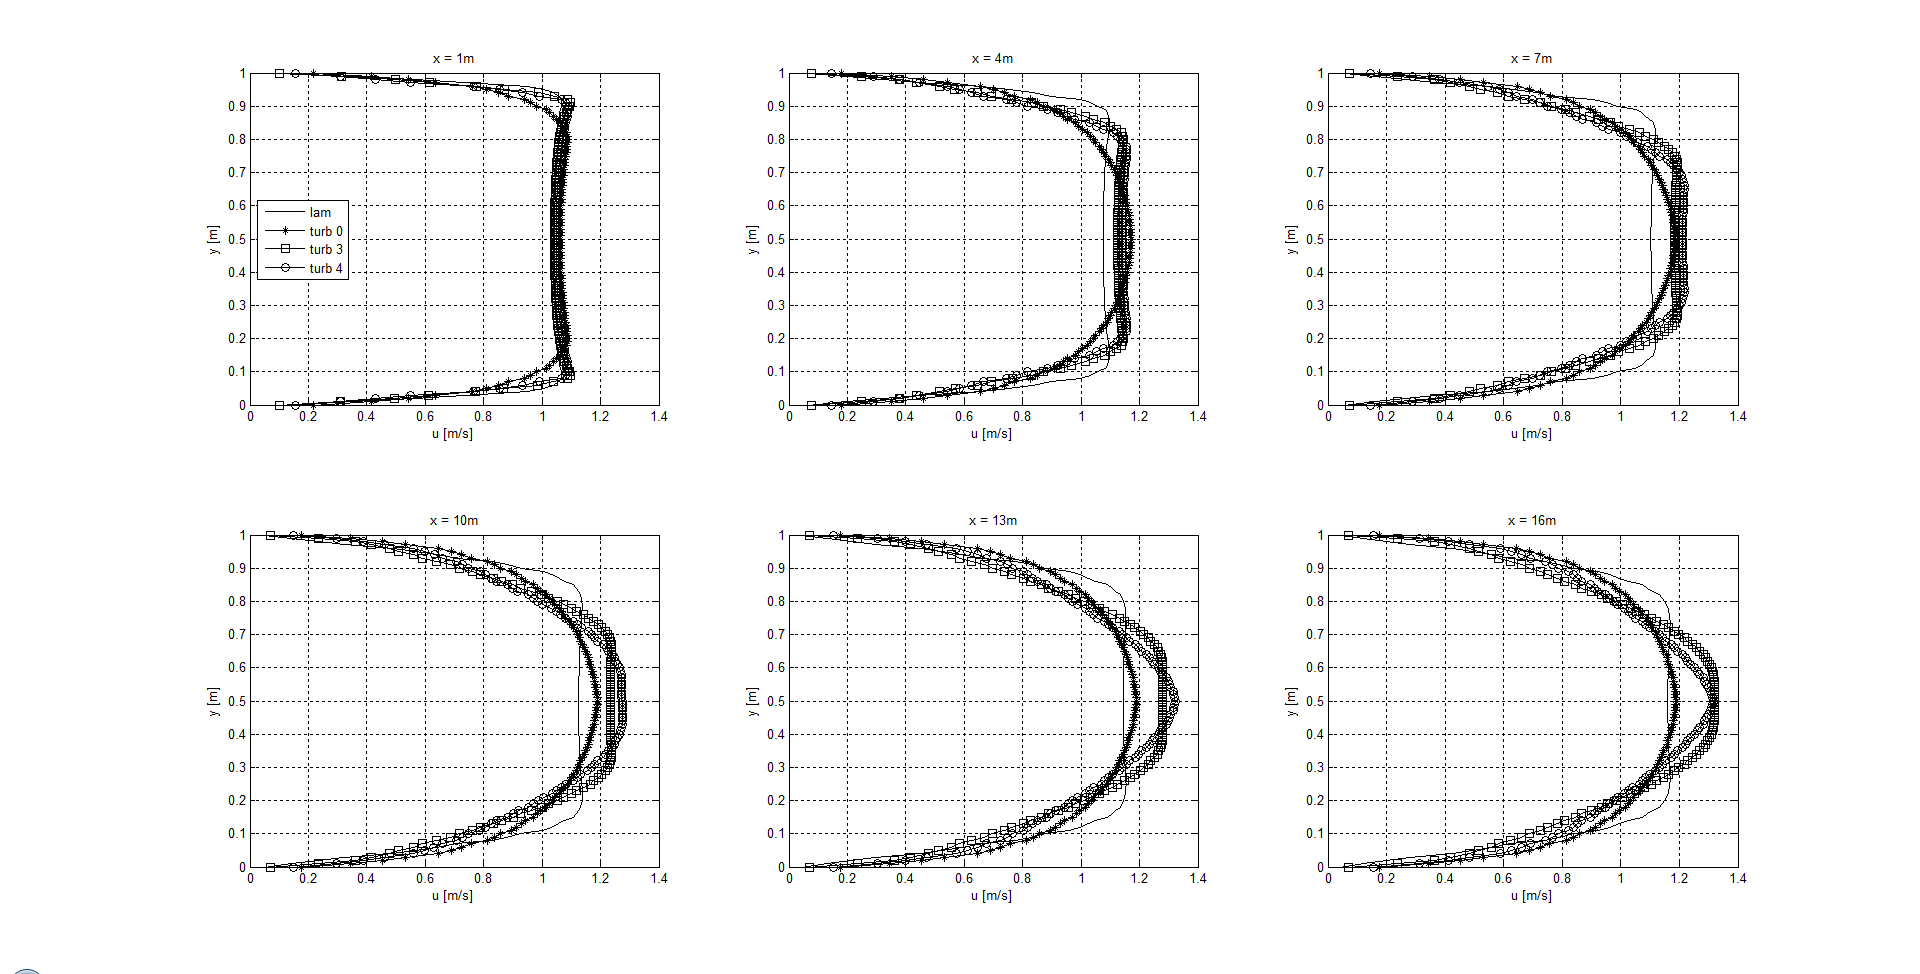
\includegraphics[trim={5cm 1.5cm 4cm 1.5cm},clip,angle=90,origin=c, width=0.8\textwidth]{yu}
    \caption{Development of the velocity profile for different $\nu_t$-limiters (uniform inlet profile)}
    \label{fig:devel}
\end{figure}

\clearpage

%\begin{figure}
%    \centering
%    \def\svgwidth{100pt}
%    \input{svg/stencils.pdf_tex}
%\end{figure}

\clearpage

\newcommand{\eqvd}{\stackrel{\mathrm{2D}}{=}}
\newcommand{\eqvdd}{\stackrel{\mathrm{3D}}{=}}

\section*{Appendix}\label{sec:appendix}
\begin{landscape}
Stencils for momentum equation in x-direction:
\begin{align*}
\left[ \abl{}{x}\left( \nu^*\abl{u}{x} \right) \right]_{i,j,k}&\eqvd
\frac{2}{\delta x_{i,j,k}+\delta x_{i+1,j,k}}
\left(
\nu^*_{i+1,j,k}\cdot\frac{u_{i+1,j,k}-u_{i,j,k}}{\delta x_{i+1,j,k}}
-
\nu^*_{i,j,k}\cdot\frac{u_{i,j,k}-u_{i-1,j,k}}{\delta x_{i,j,k}}
\right)
%
%
%
%
\\
\left[ \abl{}{y}\left( \nu^*\abl{u}{y} \right) \right]_{i,j,k}&\eqvd
\frac{1}{\delta y_{i,j,k}}
\left(
\nu^*_{i+\frac{1}{2},j+\frac{1}{2},k}\cdot\frac{2 \cdot (u_{i,j+1,k}-u_{i,j,k})}{\delta y_{i,j,k}+\delta y_{i,j+1,k}}
-
\nu^*_{i+\frac{1}{2},j-\frac{1}{2},k}\cdot\frac{2\cdot(u_{i,j,k}-u_{i,j-1,k})}{\delta y_{i,j-1,k}+\delta y_{i,j,k}}
\right)
%
%
%
%
\\
\left[ \abl{}{z}\left( \nu^*\abl{u}{z} \right) \right]_{i,j,k}&\eqvdd
\frac{1}{\delta z_{i,j,k}}
\left(
\nu^*_{i+\frac{1}{2},j,k+\frac{1}{2}}\cdot\frac{2 \cdot (u_{i,j,k+1}-u_{i,j,k})}{\delta z_{i,j,k}+\delta z_{i,j,k+1}}
-
\nu^*_{i+\frac{1}{2},j,k-\frac{1}{2}}\cdot\frac{2\cdot(u_{i,j,k}-u_{i,j,k-1})}{\delta z_{i,j,k-1}+\delta z_{i,j,k}}
\right)
%
%
%
%
\\
\left[ \abl{}{y}\left( \nu^*\abl{v}{x} \right) \right]_{i,j,k}&\eqvd
\frac{1}{\delta y_{i,j,k}}
\left(
\nu^*_{i+\frac{1}{2},j+\frac{1}{2},k}\cdot\frac{2 \cdot ( v_{i+1,j,k}- v_{i,j,k})}{\delta x_{i,j,k}+\delta x_{i+1,j,k}}
-
\nu^*_{i+\frac{1}{2},j-\frac{1}{2},k}\cdot\frac{2 \cdot ( v_{i+1,j-1,k} - v_{i,j-1,k})}{\delta x_{i,j-1,k}+\delta x_{i+1,j-1,k}}
\right)
%
%
%
%
\\
\left[ \abl{}{z}\left( \nu^*\abl{w}{x} \right) \right]_{i,j,k}&\eqvdd
\frac{1}{\delta z_{i,j,k}}
\left(
\nu^*_{i+\frac{1}{2},j,k+\frac{1}{2}}\cdot\frac{2 \cdot ( w_{i+1,j,k}- w_{i,j,k})}{\delta x_{i,j,k}+\delta x_{i+1,j,k}}
-
\nu^*_{i+\frac{1}{2},j,k-\frac{1}{2}}\cdot\frac{2 \cdot ( w_{i+1,j,k-1} - w_{i,j,k-1})}{\delta x_{i,j,k-1}+\delta x_{i+1,j,k-1}}
\right)
\\
\end{align*}
\begin{figure}[htbp]
\begin{minipage}{0.49\textheight}
Stencils for momentum equation in y-direction:
\begin{align*}
\left[ \abl{}{x}\left( \nu^*\abl{v}{x} \right) \right]_{i,j,k}&\eqvd ...
%
%
%
%
\\
\left[ \abl{}{y}\left( \nu^*\abl{v}{y} \right) \right]_{i,j,k}&\eqvd ...
%
%
%
%
\\
\left[ \abl{}{z}\left( \nu^*\abl{v}{z} \right) \right]_{i,j,k}&\eqvdd  ...
%
%
%
%
\\
\left[ \abl{}{x}\left( \nu^*\abl{u}{y} \right) \right]_{i,j,k}&\eqvd  ...
%
%
%
%
\\
\left[ \abl{}{z}\left( \nu^*\abl{w}{y} \right) \right]_{i,j,k}&\eqvdd ...
\\
\end{align*}
\end{minipage}\qquad\qquad\qquad\qquad\qquad\qquad\qquad\qquad
\begin{minipage}{0.49\textheight}
Stencils for momentum equation in z-direction:
\begin{align*}
\left[ \abl{}{x}\left( \nu^*\abl{w}{x} \right) \right]_{i,j,k}&\eqvdd ...
%
%
%
%
\\
\left[ \abl{}{y}\left( \nu^*\abl{w}{y} \right) \right]_{i,j,k}&\eqvdd ...
%
%
%
%
\\
\left[ \abl{}{z}\left( \nu^*\abl{w}{z} \right) \right]_{i,j,k}&\eqvdd ...
%
%
%
%
\\
\left[ \abl{}{x}\left( \nu^*\abl{u}{z} \right) \right]_{i,j,k}&\eqvdd ...
%
%
%
%
\\
\left[ \abl{}{y}\left( \nu^*\abl{v}{z} \right) \right]_{i,j,k}&\eqvdd ...
\\
\end{align*}
\end{minipage}
\end{figure}



\end{landscape}


\clearpage

\subsubsection*{Notes}
\noindent Be aware that the implemented method does not produce the same results for laminar flow ($\nu_T=0$) on a stretched mesh as the original implementation. This is due to a slight difference in the definition of the stencils.

\vspace{0.5cm}

\noindent\textbf{Method 1 (original)}
\begin{align*}
\left[ \abl{}{y}\left( \abl{u}{y} \right) \right]_{i,j,k}&=
\new{
\frac{2}{\delta y_{i,j,k}^=/2}
}
\cdot
\left(
\frac{u_{i,j+1,k}}{\delta y_{i,j,k}^+}
-
u_{i,j,k}\left(
\frac{1}{\delta y_{i,j,k}^-}
+
\frac{1}{\delta y_{i,j,k}^+} \right)
+
\frac{u_{i,j-1,k}}{\delta y_{i,j,k}^-}
\right)
\end{align*}
rewritten (as in the code):
\begin{align*}
\left[ \abl{}{y}\left( \abl{u}{y} \right) \right]_{i,j,k}
&=
4
\cdot
\left(
\frac{u_{i,j+1,k}}{\delta y_{i,j,k}^+\cdot \delta y_{i,j,k}^=}
-
\frac{
u_{i,j,k}
}{
\delta y_{i,j,k}^-\cdot \delta y_{i,j,k}^+
}
+
\frac{u_{i,j-1,k}}{\delta y_{i,j,k}^-\cdot \delta y_{i,j,k}^=}
\right)
\end{align*}

\vspace{0.5cm}

\noindent\textbf{Method 2 (new)}\\
\noindent($\nu^*$ considered as constant, so that it can be neglected)
\begin{align*}
&\left[ \abl{}{y}\left( \abl{u}{y} \right) \right]_{i,j,k}=
\new{
\frac{2}{\delta y_{i,j,k}}
}\cdot
\left(
\frac{u_{i,j+1,k}}{\delta y_{i,j,k}^+}
-
u_{i,j,k}\left(
\frac{1}{\delta y_{i,j,k}^-}
+
\frac{1}{\delta y_{i,j,k}^+} \right)
+
\frac{u_{i,j-1,k}}{\delta y_{i,j,k}^-}
\right)
\end{align*}

\vspace{0.5cm}

\noindent For a stretched mesh (tanh) and a parabolic flow field (n=2), the method 1 produces exact results in contrast to method 2. Method 2 shows a quadratic convergence. This method was used because the first derivatives were needed at the nodes to be able to multiply with matching $\nu_t$.

\vfill
with:
\begin{align*}
\delta y_{i,j,k}^- &= \delta y_{i,j-1,k}+\delta y_{i,j,k} \\
\delta y_{i,j,k}^+ &= \delta y_{i,j+1,k}+\delta y_{i,j,k} \\
\delta y_{i,j,k}^=&=\delta y_{i,j,k}/2+ \delta y_{i,j,k}+\delta y_{i,j,k}/2
\end{align*}

\end{document}
